\documentclass[12pt]{article}
 \usepackage[hcentering,bindingoffset=20mm]{geometry}
 \usepackage{placeins}
 \usepackage[numbib]{tocbibind}
 \usepackage{rotating}
\usepackage[square,sort,comma,numbers]{natbib}
 \usepackage{graphicx}
 \usepackage{tabularx}
 \linespread{1.3}
 \usepackage{gensymb}
\usepackage{longtable}
 \usepackage{lscape}
 \usepackage{url}
 \addtolength{\textwidth}{2cm}
 \addtolength{\hoffset}{-1cm}
 
 
 \addtolength{\textheight}{2cm}
 \addtolength{\voffset}{-1cm}
 \setlength{\parindent}{0pt}
 
\title{Redefinition of the evolutionary relationships within the gonyaulacales - wrangling paralogy in transcriptomes for phylogenetics. $^{1}$}
\author{Key words: Bayesian inference, gonyaulacales, phylogenetics, transcriptomics}
\date{}

\begin{document}
\maketitle
\paragraph{}Anna Liza Kretzschmar$^{2}$\\
Climate Change Cluster (C3), University of Technology Sydney, Ultimo, 2007 NSW, Australia, anna.kretzschmar@uts.edu.au
\paragraph{}Aaron Darling \\
Ithree institute (i3), University of Technology Sydney, Ultimo, 2007 NSW, Australia
\paragraph{}Mathieu Fourment \\
Ithree institute (i3), University of Technology Sydney, Ultimo, 2007 NSW, Australia
\paragraph{}Shauna Murray\\ 
Climate Change Cluster (C3), University of Technology Sydney, Ultimo, 2007 NSW, Australia
\newpage
\section{Abstract}
\newpage

\section{Introduction}

% AD 131217: the "NGS advances" opener is a bit cliche these days, but ok as a placeholder
Advancement in next generation sequencing has heralded a new era for investigating the evolutionary relationships between organisms. 
% AD 131217: don't we use models as a point of reference to develop understanding of specific biological parts and functions, which we then extrapolate to relatives via homology?
The main focus has been on model organisms to infer the genetic make up of similar taxa. 
Model organisms are usually characterised by a reference genome and established protocols for working with. 
In the eukaryotic world, these well established model organisms only cover a predicted xx \% of known taxa. 
With the reduction in sequencing cost, increasingly large transcriptomic datasets are available for non-model organisms without reference genomes. 
% AD 131217: I'm not sure I understand what the following sentence means. I think you will have to be more explicit about what makes non-models difficult to analyse
Working with these taxa can pose obstacles for evolutionary inference when they do not satisfy the model selection or processing assumptions commonly attributed to model organisms. Frequent issues arise from:\\
% AD 131217: It would help to say more specifically that these are problems for species tree inference
1) Selection of paralogs. If genes with different evolutionary histories are selected, the gene tree will not reflect the history of either paralog and be nonsensical for species tree inference; 
2) Concatenation of genes. Can be statistically inconsistent estimator of the species tree due to incomplete lineage sorting and concatenation acting as imperfect estimator of species tree topology \cite{roch2015likelihood}; and 
3) Inference of model adequacy from bootstrap values. Kubatko et al. (2007) demonstrated high bootstrap support under maximum likelihood inference for incorrect species trees with concatenated gene sets as input \cite{kubatko2007inconsistency}. 
% AD 131217: the above passage is good.

% AD 131217: might say "attempts to address" since it's not clear to what extent they have been fully addressed
As high bootstrap values are often used as an indicator for robust species topology resolution, this fallacy is particularly problematic if the reader/operator is unfamiliar with the statistical phenomenon.\\
In this study we aim to build a bioinformatic pipeline that attempts to addresses the issues of paralogy when processing transcriptomic data from non-model organisms, utilises alternative methods to both concatenation and maximum likelihood inference. 
% AD 131217: I think most people write RNAseq or RNA-seq
Specifically, the pipeline assembles RNA seq datasets, identifies and extracts single copy genes across input taxa with extensive paralogy, and runs Bayesian inference phylogenetics. 
Finally, to apply the pipeline to the historically difficult order Gonyaulacales (phylum: Dinoflagellata) which are notorious for the issues that the pipeline seeks to address.\\
% AD 131217: suggest starting a new \subsection{} here
%protists and environmental importance
\subsection*{Gonyaulacales - a phylogenetic obstacle course}
Dinoflagellates represent an ancient lineage on the eukaryotic branch of life. 
They play a role in several important ecological processes, as members are represented in aquatic environments, where the cover a diverse niches such as symbionts, parasites and some taxa can cause harmful algal blooms through proliferation and/or neurotoxin production.
While the evolutionary relationship of most orders within the dinoflagellates has been estimated with reasonable certainty, one order has consistently escaped scrutiny - the gonyaulacales. 
Analyses for this order commonly combined concatenation and maximum likelihood approaches, which yielded long branch attraction, low confidence values and inconsistent taxon resolution. 
Improving upon the species the evolution of the gonyaulaceles has implications for environmental disease monitoring, as neurotoxin production is prevalent in this order. 
Specifically the ciguatoxins produced by some \emph{Gambierdiscus} spp. are of interest as the causative agent of ciguatera fish poisoning, a neglected tropical disease with high associated morbidity.%, which is predicted to increase in prevalence with the advent of climate change.


\newpage

\section{Materials and methods}
\subsection*{Culture conditions}
\FloatBarrier
Cultures were isolated from locations as per Table ~\ref{tbl:strainTable} and clonalal cultures established by micropipetting single cells through sterile seawater. 

\begin{table}
\caption{Culturing conditions for species processed for this study.}
\label{tbl:strainTable}
\begin{tabular}{ | p{3cm} | p{2.5cm} | p{1.5cm} | p{5.3cm} |}
\hline
\textbf{Species} & \textbf{Strain}& \textbf{Temp} & \textbf{Source location} \\
%\hline
%\textit{Coolia malayensis}&MAB&& \\
\hline
\textit{Gambierdiscus carpenteri}&UTSMER9A&17&Merimbula, AU\\
\hline
\textit{Gambierdiscus lapillus}&HG4&27&Heron Island, AU\\
\hline
\textit{Gambierdiscus polynesiensis}&CG15&27&Rarotonga, COK\\
\hline
\textit{Gambierdiscus} cf. \textit{silvae}&HG5&27&Heron Island, AU\\
\hline
%\textit{Ostreopsis ovata}&HER27&&\\
%\hline
%\textit{Ostreopsis rhodesae}&HER26&&\\
%\hline
%\textit{Ostreopsis siamensis}&BH1&&\\
%\hline
\textit{Thecadinium kofoidii}&THECA&18&Gordons bay, Sydney, AU\\
\hline
\end{tabular}
\end{table}
\FloatBarrier
 \subsection*{RNA isolation}
%\textit{Coolia malayensis}, \textit{Ostreopsis ovata}, \textit{Ostreopsis rhodesae} and \textit{Ostreopsis siamensis} were processed as per Ref ARJUN.
\emph{Gambierdiscus} spp. and \emph{Thecadinium kofoidii} were harvested during late exponential growth phase by filtration onto 5 $\mu$m SMWP Millipore membrane filter (Merck, DE) and washed off with sterile seawater. 
Cells were pelleted via centrifugation (make of centrifuge) for 10 minutes at 350 rcf. 
Supernatant was decanted and 2ml of TRI Reagent (Sigma-Aldrich, subsidiary of Merck, DE) was added to the pellet and vortexed till dissolved. 
Samples were split in two and transferred to 1.5ml eppendorf tubes. 
Cellular thecae were ruptured by three rounds of freeze-thaw, with tubes transferred between liquid Nitrogen and 95 $^{\circ}$C. 
RNA was extracted as per protocol for TRI Reagent. 
RNA elute was purified with the RNeasy RNA clean up kit EXACT NAME as per protocol(Qiagen). 
DNA was digested with TurboDNAse (Life technologies, subsidiary of Thermo Fischer scientific, AU). 
RNA was quantified with Nanodrop 2000 (XXX) and frozen at -80 $^{\circ}$C until sequencing.
 
\subsection*{Library preparation and Sequencing}
The quality of samples was assessed via Agilent 2100 Bioanalyzer. 
Paired-end sequencing was performed on NextSeq 500 High Output was conducted by Ramaciotti center (UNSW, AU) with 75bp insert size for \emph{G. lapillus} and \emph{G.} cf. \emph{silvae}; and 150bp inserts for \emph{G. carpenterii}, \emph{G. polynesiensis} and \emph{T.} cf. \emph{kofoidii}.


%\subsection*{Transcriptomes}
%\emph{Coolia malayensis}, \emph{Gambierdiscus carpenteri}, \emph{Gambierdiscus lapillus}, \emph{G. polynesiensis}, \emph{Gambierdiscus} cf. \emph{silvae} \emph{Ostreopsis ovata}, \emph{Ostreopsis rhodesae}, \emph{Ostreopsis siamensis} and \emph{Thecadinium} cf. \emph{kofoidii} were grown in F/10 medium at 25 - 27 degrees celcius, except for \emph{T.} cf. \emph{kofoidii} which was grown at 18 degrees celcius, and cells were harvested via centrifugation at 350 rcf for 10 minutes at late exponential phase. Trizole was directly added to cells, cells were opened by three cycles of freezing in liquid nitrogen and thaw at 95 degrees celcius, then RNA was extracted as per reccomendation for Trizole by the manufacturers. Quality of RNA was screened by Agilent Bioanalyzer and paired-end sequencing was performed on NextSeq 500 High Output by Ramaciotti, UNSW. \emph{G. lapillus} and \emph{G.} cf. \emph{silvae} sequencing libraries were created with 75bp insert size; \emph{G. carpenterii}, \emph{G. polynesiensis} and \emph{T.} cf. \emph{kofoidii} sequencing libraries were created with 150bp inserts.
\subsubsection*{Publically available transcriptome libraries}
\emph{Gambierdiscus excentricus} VGO790 transcriptome was downloaded from NCBI under accession ID SRR3348983 \cite{kohli2017role}. 
\textit{Coolia malayensis}, \textit{Ostreopsis ovata}, \textit{Ostreopsis rhodesae} and \textit{Ostreopsis siamensis} sequencing libraries were aquired from Arjun Verma (Verma 2018, in prep). 
RNA seq libraries for all remaining transcriptomes were generated by, and downloaded from, the Marine Microbial Eukaryote Transcriptome Sequencing Project \citep{keeling2014marine}.

\subsection*{Pipeline}
The pipeline is packaged in the Nextflow language \cite{nextflow} for streamlined transferal between high powered computing clusters. 
The workflow is separated into part 1 and part 2, and modules within the pipeline are written in bash an Python 2.7 \cite{python}, including the pandas module \cite{pandas}, and can be found on github. The pipeline was run on the Genomics Virtual Lab (GVL) \cite{afgan2015genomics} inside the National eResearch Collaboration Tools and Resources (NeCTAR) research cloud, an initiative by the National Research Infrastructure for Australia (NCRIS) \cite{nectar}.
\subsubsection*{Pipeline part 1}
The input to pipeline 1 were the individual RNA sequencing library which is the processed through FastQC \cite{fastqc} for quality assurance, sequences are trimmed with Trimmomatic \cite{bolger2014trimmomatic} and assembled with Trinity v2.4.0 \cite{haas2013novo}. 
Assemblies were then processed with BUSCO2 with the protist specific library \cite{simao2015busco}.
The RNA libraries with 150bp inserts generated as part of this study were also subjected to Digital Normalization \cite{diginorm} to pool identical transcripts before assembly.                                                                                                                                                                                                                                                                                                                                                                                                                                                                                                                                                                                                                                                                                                                                                                                                                                                                                                                                                                                                                                                                                                                                                                                                                                                                                                                                           
\subsubsection*{Pipeline part 2}
The input to pipeline 2 was the output of BUSCO2, where all complete single copy genes were identified per transcriptome. 
Any genes that were present in at least 75 \% the transcriptomes were indexed, the corresponding contig extracted from the assemblies, aligned with hmmer3.1b2 \cite{eddy2015hmmer} and unaligned regions trimmed.
\subsection*{Phylogenetic inference}
The pipeline output was processed on the University of Technology's High-powered computing cluster.
Species evolutionary inference was based on Bayesian probability with the *BEAST2 model in BEAST2 \cite{bouckaert2014beast}. 
The analysis was performed under the WAG substitution model \cite{whelan2001general} with a Gamma distribution for four rate categories. 
A random local clock was employed \cite{drummond2010bayesian}. 
Posterior distributions of parameters were approximated after 300,000,000 generations of MCMC runs with 4 heated and one cold chain, sampled ever 5,000 generations  with a burn in of 15\%. 
The inference was run four times to compare convergence parameters, then log and tree files were merged. 
Inference was run using BEAGLE \cite{ayres2011beagle} on GPU.

\subsection*{Assembly analysis}
Contigs from assemblies from pipeline part 1 were clustered with CD-HIT with the command cd ..
cd-hit \cite{fu2012cd}, transdecoder %\cite{haas2016transdecoder}, cd-hit, get_homologs \cite{contreras2013gethom}, interproscan \cite{quevillon2005interproscan}
%BLAST2GO is kind of lame and takes weeks per transcriptome.. trying clustering and interpro scan instead
%searched against NCBI's non-redundant (nr) database in a BLASTx search with and E-value cut off $\leq$ 10$^{-3}$ in Blast2GO \cite{conesa2005blast2go}. 
%Mapping and annotation were performed in Blast2GO also, including gene ontology (GO) term retrieval and enzyme code determination to establish metabolic pathways though the retrieval database.
\subsection*{Inference run time comparison}
A subset of 14 taxa was selected for a comparison between CPU and GPU inference run time comparison. 
The transcriptome libraries were fed through the pipeline as described, which was set to extract single copy genes present in all of the taxa. 
The resulting alignments were run on *BEAST either on the CPU or GPU.

\newpage
\section{Results}
\subsection*{Transcriptomes overview}
Sequencing of transcriptomes for \emph{Gambierdiscus} spp. and \emph{T. kofoidii} generated datasets ranging in size fro, XX million to XX million reads, resulting in assembled sequence data XX to XX Mbp in size, which corresponded to XX to XX assembled contigs (table ~\ref{tbl:asmstats}). 
Approximately XX\% to XX\% predicted to be protein coding sequences. %Transdecoder stats?
In all five transcriptomes the complete protein coding pathways were present. %CHEXCK
%work mothur for this
\FloatBarrier
\begin{longtable}{  | p{3cm} |p{2cm} | p{2cm} | p{2cm} | p{2cm} | p{2cm} |}
\caption{Summary of transcriptome sequencing and assembly statistics.}\\
\hline
\label{tbl:asmstats}
\emph{Sequences:}&\emph{G. carpenteri}&\emph{G. lapillus}&\emph{G. polynesiensis}&\emph{G.} cf. \emph{silvae}&\emph{T. kofoidii}\\
\hline
 \multicolumn{6}{| c |}{Sequencing}\\
 \hline
\textbf{SRA accession}&&&&&\\
\hline
\textbf{Raw sequencing reads}&&&&&\\
\hline
 \multicolumn{6}{| c |}{Assembly}\\
 \hline
 \textbf{Contigs}&&&&&\\
\hline
\textbf{Average length (bp)}&&&&&\\
\hline
\textbf{Range of contigs length (bp)}&&&&&\\
\hline
\textbf{GC content/N50?}&&&&&\\
\hline
  \multicolumn{6}{| c |}{Transcript clustering \& annotation}\\
\hline
\textbf{\# clusters}&&&&&\\
\hline
\textbf{with protein functional domains}&&&&&\\
\hline
%\textbf{with full annotations}&&&&&\\
%\hline
%\textbf{with Enzyme Codes}&&&&&\\
%\hline
%\textbf{mapped to KEGG pathways}&&&&&\\
%\hline
\end{longtable}

\subsection*{Transcripome stuff}
Assemblies for all transcriptome datasets used in this study were channeled through the pipeline. The single copy genes acquired though the BUSCO hmmer libraries curated for protists are reported in Table ~\ref{tbl:Transcriptomes} out of the total xx genes searched for, as well as accession numbers and identifiers for each transcriptome.
\FloatBarrier
\begin{longtable}{  | p{3cm} |p{4.5cm} | p{2cm} | p{2cm} | p{3cm} |}
\caption{Transcriptomes used for study along with taxonomic placement at family level and source. Family level placement derived from algaebase. MMETSP abbreviation for marine Microbial eukaryotic transcriptome sequencing project, by Moore Foundation.}\\
\hline
\label{tbl:Transcriptomes}
\textbf{Family}&\textbf{Species}&\textbf{Strain}&\textbf{BUSCO single complete}&\textbf{Source}\\
\hline
 \multicolumn{5}{| c |}{Gonyaulacales transcriptomes}\\
    \hline
   Ceratiaceae&\emph{Ceratium fusus}&PA161109&81&MMETSP1074 \citep{keeling2014marine}\\
        \hline
  Crypthecodiniaceae&\emph{Crypthecodinium cohnii}&Seligo&98&MMETSP0326\_2 \citep{keeling2014marine}\\
        \hline
    &\emph{Alexandrium catenella}&OF101&74&MMETSP0790 \citep{keeling2014marine}\\
        \hline
    &\emph{Alexandrium monilatum}&JR08&74&MMETSP0093 \citep{keeling2014marine}\\
        \hline
&\emph{Pyrodinium bahamense}&pbaha01&89&MMETSP0796 \citep{keeling2014marine}\\
        \hline
Gonyaulacaceae&\emph{Coolia malayensis}&MAB&100&This study\\
\hline
&\emph{Gambierdiscus carpenteri}&UTSMER9A&83&This study\\
\hline
&\emph{Gambierdiscus excentricus}&VGO790&83&\\
        \hline
    &\emph{Gambierdiscus lapillus}&HG4&98&This study\\
        \hline
            &\emph{Gambierdiscus polynesiensis}&CG14 really&81&This study\\
        \hline
    &\emph{Gambierdiscus} cf. \emph{silvae}&HG5&87&This study\\
        \hline
    &\emph{Gonyaulax spinifera}&CCMP409&53&MMETSP1439 \citep{keeling2014marine}\\
        \hline
%    &\emph{Lingulodinium polyedra}&CCMP1738&MMETSP1032&209&\citep{keeling2014marine}\\
 %       \hline
     &\emph{Ostreopsis ovata}&HER27&99&This study\\
     \hline
     &\emph{Ostreopsis rhodesae}&HER26&98&This study\\
     \hline
     &\emph{Ostreopsis siamensis}&BH1&98&This study\\
     \hline     
Protoceratiaceae&\emph{Protoceratium reticulatum}&CCCM535=CCMP1889&72&MMETSP0228 \citep{keeling2014marine}\\
    \hline
 &\emph{Thecadinium kofoidii}&THECA&70&This study\\
 \hline
 \multicolumn{5}{| c |}{Outgroup transcriptomes}\\
 \hline
Dinophysiaceae&\emph{Dinophysis acimunata}&DAEP01&74&MMETSP0797 \citep{keeling2014marine}\\
        \hline
Dinophyceae incertae sedis&\emph{Azadinium spinosum}&3D9&81&MMETSP1036\_2 \citep{keeling2014marine}\\
        \hline
Gymnodiniales&\emph{Karenia brevis}&CCMP2229&85&MMETSP0030 \citep{keeling2014marine}\\
    \hline
\end{longtable}

Azadinium Order Dinophyceae incerta sedis according to algaebase, gonyaulacales from NCBI taxonomy

\subsection*{Phylogeny}
The gonyaulacales resolved as a monophyletic order with three major clades, tentatively named clades I - III. PP branch support values were analyzed as follows: 1.00 was fully supported, $\geq$ 0.9 was very well supported, $\geq$ 0.8 was relatively well supported and $\leq$ 0.5 was unsupported.
The separation of clades I, II and III was fully supported, the PP within the three clades was predominantly fully or very well supported. 
The exception in clade I was the placement of \emph{O. ovata} as sister species to \emph{O. rhodesae} with a PP of 0.76. 
The exception in clade II was in \emph{G. carpenteri} placement as sister species to \emph{G. excentricus} with a PP of 0.61. In clade III, the placement of \emph{P. bahamense} as basal to the other taxa within that clade was supported with 0.57, while the split off for \emph{T. kofoidii} was relatively well supported.
The PP for the deeper branching clades was well resolved (Check). %look up terminology for this
Clade I within the gonyaulacales contains \emph{Alexandrium} spp., \emph{Coolia malayensis} and \emph{Ostreopsis} spp. 
Clade II contains \emph{Gambierdiscus} spp. as well as \emph{Pyrodinium bahamense} as sister genus. 
Clade III contains \emph{Pyrodinium bahamense}, \emph{Ceratium fusus}, \emph{Gonyaulax spinifera}, \emph{Protoceratium reticulatum} and \emph{Thecadinium kofoidii}. 
This inference suggests that \emph{O. ovata} and \emph{O. rhodeseae} are sister species with \emph{O. siamensis} diverging earlier. 
This is contrary to the \emph{Ostreopsis} species evolution in the literature to date, which is based on ribosomal genes \cite{verma2016molecular}. 
The placement of \emph{Gambbierdiscus} species from this study follows the species resolution in the literature to date \cite{kretzschmar2017characterization}. 
\emph{Crypthecodinium chonii} did not resolve within the gonyaulacales (green branch Fig. ~\ref{fig:phylo}), but clustered as an outgroup, more distant that the other outgroup taxa \emph{Azadinium spinosum}, \emph{Karenia brevis} and \emph{Dinohysis acuminata}.
%check toxin production along those branches
\FloatBarrier 
\begin{figure} 
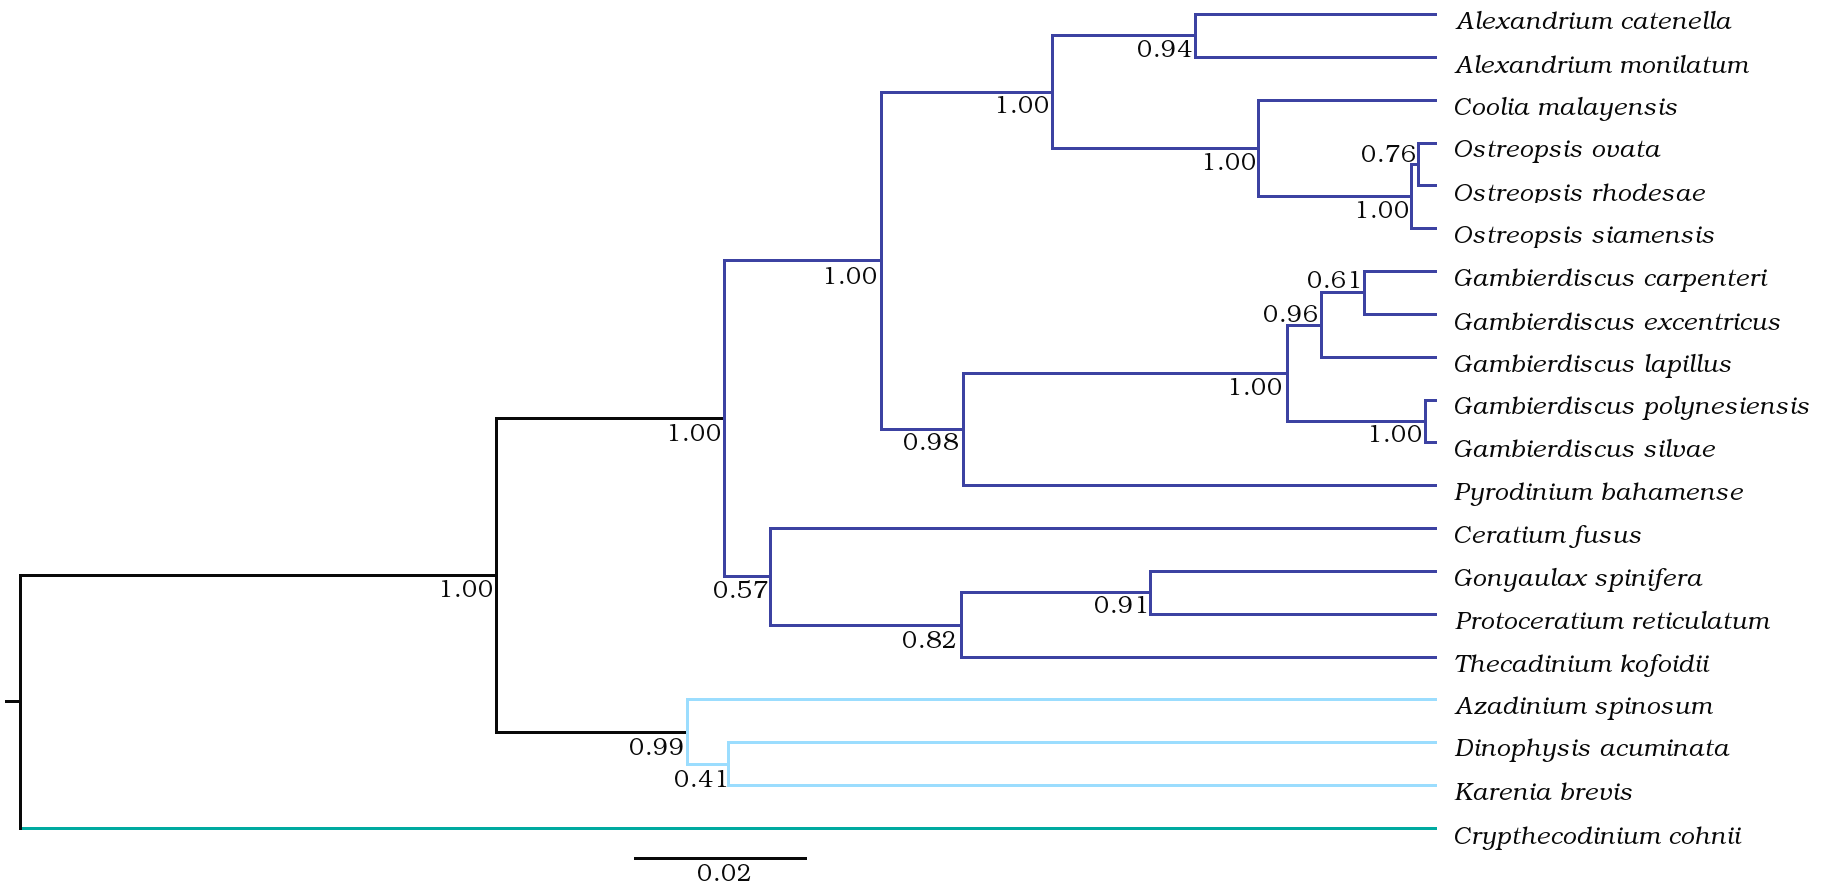
\includegraphics[scale=.25]{Aug2_20-taxa-combined-fig_MCC_trees_gimp.png} 
\caption{Phylogenetic analysis of Gonyaulacales species tree with 62 single copy genes from 20 taxa. Gonyaulacales (\#16) in purple, outgroups (\#3) in light blue and taxa \textit{incertae sedis} (\#1) in teal.} 
\label{fig:phylo}
\end{figure} 
\FloatBarrier
\newpage
\section{Discussion}
This study presents a pipeline designed to identify single copy genes in transcriptomes from taxa with extensive paralogy, extracting and aligning single copy gene sequences and running phylogenetic inference. 
The pipeline was tested on the order gonyaulacales, class Dinophyceae, with publicly available transcriptomes as well as transcriptomes presented as part of this study. 
With publicly available datasets such as the MMETSP project for marine microbes \cite{keeling2014marine}, previous data based limitations for exploring the species evolution within these abundant organisms can now be overcome. 
However, the next obstacle lies in the methodology for investigating these taxa and this is what this study seeks to address. 
The process of paralog elimination as input for species inference presented here is transparent and reproducible. 
The gonyaulacales were chosen to test the pipeline due to the size of their genomes and extensive paralogs.
This pipeline is publicly available through github and the single copy genes used to infer the species evolution in this study, as well as the log files for the *BEAST runs, are available on zenodo.
\subsection*{Phylogeny comparison to previous studies} 
As a result we present a phylogeny with good support values, a range of taxa that covers 5 of the 9 families with the gonyaulacales proposed by algaebase, which is the taxonomy authority for phycology journals, e.g. Journal of Phycology. Families not represented in this study were the Cladopyxidaceae \& Pyrophacaceae for which no transcriptome libraries were available; and Hystrichosphaeridiaceae \& Pterospermopsidaceae whose extant taxa appear to be fossils.
Rather than the five families in the gonyaulacales, this study proposes three well supported sub-clades. 
These do not correspond to previous studies, however this is likely due to: 
\subsubsection*{(1) infering species evolution from a small subset of genes such as ribosomal genes, whose evolution may not reflect that of the species.}
Using LSU or SSU rDNA regions for phylogenetics is common practice. eg XXX. 
It is important to acknowledge that these represent the evolutionary history of highly conserved genes, which does not necessarily represent the species evolution. 
Hence studies which utilise primarily rDNA genes for inferring species phylogeny run the risk of presenting the evolutionary history of rDNA genes as synonymous with species evolution.
To address this obstacle, a range of genes need to be used to infer the species evolution.
\subsubsection*{(2) concatenating the genes selected and using maximum likelihood methods for species inference.}
Concatenation of genes coupled with running maximum likelihood inference is a commonly used method as it is computationally cheap in comparison to Bayesian inference methods. 
However as demonstrated by Kubatko et al. (2007) and Roche et al. (2015), this approach is error prone and can be misleading by presenting high bootstrap values.
Phylogenies that use concatenation with ML XXX
This issue is addressed in this study by running Bayesian inference under a multi-species coalescence process.
\subsubsection*{(3) quantity of taxa or quality of transcriptome assemblies.}
Several studies have inferred the evolutionary relationship within the gonyaulacales as part of larger studies around the dinoflagellates, and as such the number of taxa from within the gonyaulacales is too limited to speculate on the families or clades within the order. Eg XXX
Since the publicly available MMETSP datasets, several studies have utilised a broader range of taxa to explore gonyaulacales evolution. 
However, these have relied on the assemblies supplied by the project. 
The stringency of quality trimming of RNA-seq libraries prior to assembly plays a role in the number of unique contigs recovered and the subsequent assembly quality of transcriptomes. 
Commonly high stringency is favored, however MacManes (2014) found that this can be detrimental to the assembly and the quality cut off scores used in this pipeline were in recommendation with that study \cite{macmanes2014optimal}.
Regarding the transcriptome assembly method, Cohen et al. evaluated the publicly available assemblies from MMETSP, compared to processing and re-assembly with Trinity \cite{cohen-reass}. 
Cohen et al. demonstrated that while the raw data available from the MMETSP project is awesome, the assembly method has become outdated. 
% check veracity of statement: Further, the assembly method used can result in the assembly of paralogs into a single contig, giving the illusion of a single copy gene while actually representing hybrids. 
To address this problem, trimming and assembly of RNA-seq libraries using Trimomatic and Trinity respectively are integral to the pipeline.
%Explain here with Cohen's BUSCO scores, or compare to own? Hence, it is imperative to re-assembly the transcriptome libraries before searching for single copy genes or paralogs.
Studeis XXX
\subsubsection*{(4) selection of paralogs to infer species evolution.}
%Other studies... long branch attraction?
Selection of paralogs for species inference is highly problematic as it will present an arbitrarily divergent gene history as input. 
This problem is particularly present in the dinoflagellates and gonyaulacales due to the frequent gene duplication discussed previously. %is it?
Only one other study by Price et al. (2017) seeks to address this by purportedly selecting single genes as input. 
However there are several issues with the study presented by Price et al \cite{price2017robust}. 
The assemblies used are from the MMETSP project, which are problematic as mentioned in (3) as they can present single copy genes which are hybrids of paralogs. 
Hence the selection of single copy genes as input to the species evolution inference, is dubious. 
Further, when the scripts for selecting single copy genes were requested in order to replicate their study, the authors were unable to supply any record of how the genes were attained hence it was not possible to examine the parameters that went into identifying single copy genes. 
Lastly, the genes were concatenated and the evolutionary relationships were inferred using ML. While the bootstraps are well supported, this could very well be due to the methodology problems outlined in (2).
The difference in topology between topologies presented by Price et al. and this study (Fig. ~\ref{fig:tangle}), is lies in the organization of sister taxa 

\FloatBarrier 
\begin{figure} 
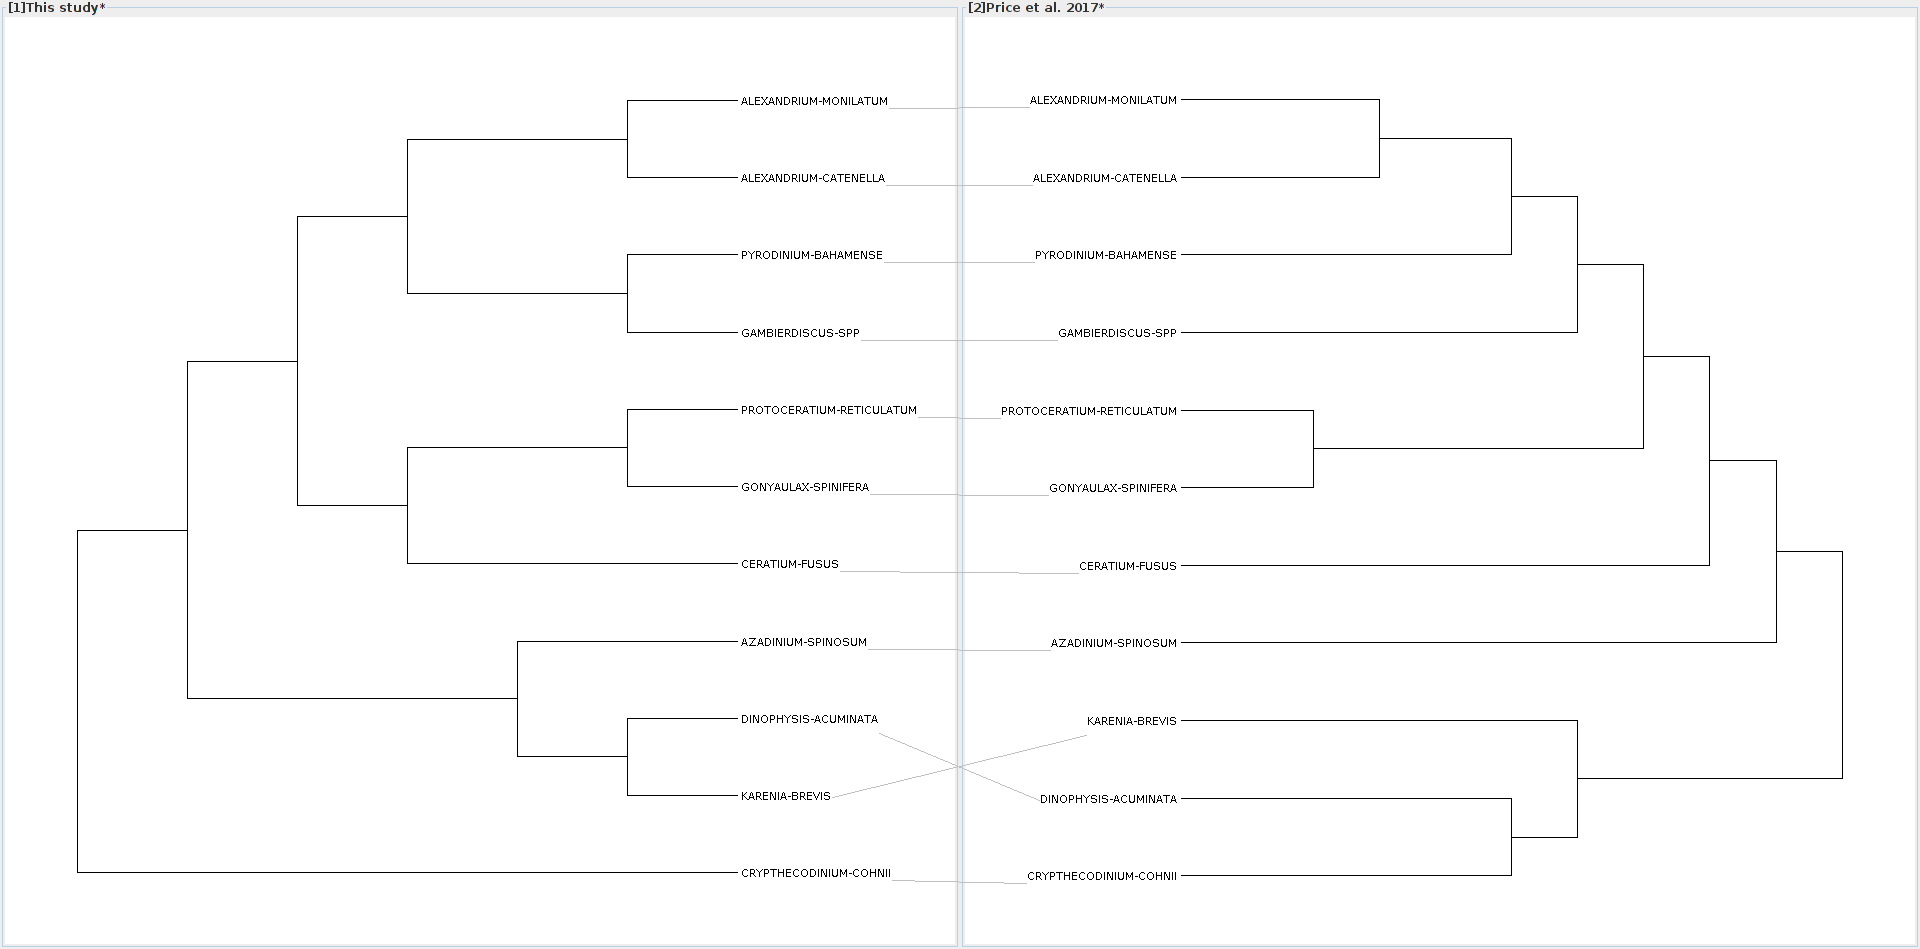
\includegraphics[scale=.23]{Price-comparison.png} 
\caption{Tanglegram of topology presented in this study (a) and Price et al. (2017) (b). Taxa uncommon to both studies not shown.} 
\label{fig:tangle}
\end{figure} 
\FloatBarrier


\subsection*{Comparison to Mona's proposal}

Historically, the evolutionary inference for organsims from this group have been 
Dinoflagellates are renowned for their large genomes and paralogy, which is why historically the evolutionary inference for them has been shithouse. With the recent completion and public availability of the MMETSP database, transcriptomes to investigate the evolutionary relationship for marine protists has become possible. And several studies have looked at the evolutionary relationships. While most clades of the dinoflagellates have been relatively well worked out, the gonyaulacales have been recalcitrant. So these have been of particular interest, especially as many of the taxa produce polyketide toxins that cause seafood intoxications globally. However, now that the transcriptomes are available, it's crucial to develop robust and reproducible methods to analyse the data
\subsection*{Phylogeny}
- differences between ML and BI analyses incl tanglegram
- literature on concatenation problem, incl. BS misleading (Kubatko 07, Roche 15)
- assembly diffs if transrate pans out
- something about single copy genes for paralog riddled taxa

\subsection*{Diff to previous gonyaulacales phylogenies}

The gonyaulacales phylogenies pre-dating this study differ extensively from the results presented here. As established, this is likely due to the methodologies used. A further factor is the available data for evolutionary inference. Before the MMETSP project, studies would either utilise a samll number of taxons with in depth sequencing, or taxons to cover the proposed family structure for this order but utulise only a small number of genes for investigation. The MMETSP database has allowed protists to join many other organisms on the big data set stage. With the access to data no longer as the limiting factor for analyses, the focus must now fall on the methods used to explore this data.
Several studies have been oublished employing the MMETSP database content since the project has gone live, for both direct exploration of the availavble data as well as supplementing trnascriptomes to answer questions. Arguably, there is a dosconnect between bioinformaticians, computer scientists and biologists which is well showcased in this area. The tennets of reproducible bioinformatics is hinged on open access software, as well as documentation, a sound understanding of the methods employed and best practices vs. computational trade-offs in analyses. As the gonyaulacales have proven a recalcitrant order for which to infer evolution, with a number of genetic peculiarities which make nalyses particularly prone to errors, this is an excellent case study.
The phylogeny presented by Price t al. 2017 is based on a similar assumption as this study - that single copy genes are the key to circumventing the issue of paralogy when selecting genes of interest. However, the methodology for identifying and selecting these single copy genes is not included in the publication. Further, contact with the author established that there was no script or documented steps for the pipeline that the authors executed. The bootstrap values for the resulting phylogeny are remarkably well supported, however without transparency for the gene selection for which genes were included or how the sequences were manipulated prior to phylogenetic inference the bootstrap values could simply be a case of the xxx phenomenon described by Kubatko et al. REF.
In Jackounevceck et al.'s 2016 study, the gonyaulacales phylogeny was part of the greater analyses around the phylum ?????, using the MMETSP transcriptomes to infer a number of evolutionary trends such as thecate evolution XXXXXX. NEED TO LOOK THIS HSIT UP AGAIN

The dominant method for established species trees is based on SSU and LSU rDNA sequences, usually within the genus and a small number of outgroups. The prevailing problem with this approach is that that deeper branches bwetween genera or higher taxonomic points is not well explored. Interestingly, the phylogenetic resolution of two genera with the highest species coverage, \emph{Gambierdiscus} and \emph{Ostreopsis}, did not mimic the resolution established in the literature within either genus. This is likely due to the rDNA sequences targeted for the usual studies reflect the evolution of that particular gene region, rather than the species evolution itself. However the arrangement of sister species for both \emph{Gambierdiscus} and \emph{Ostreopsis} matched that of the ketosynthase module of polyketide synthase complexes, which are thought to be involved in polyketide toxin production (Unpublished A. Kretzschmar; pers. comm. A. Verma). 

The use of a concatenation approach for the gene regions examined, coupled with ML for the inference, is commonly used in the literature. COncatenation as an approach suffers from a number of issues. The individual genes' evolutionary history can be quite distinct from the overall species evolution, yet they are treated as sharing the same evolutionary history, along with the rate in which the genes differentiated. This leads to a number of pitfalls (for details please see XXX), such as long branch attraction and incomplete lineage sorting, both which appear evident in studies using these methods for the gonyaulacales phylogeny elucidation (REF).
The BI matrix approach was chosen for this study to directly address these pitfalls. The resulting phylogeny (Fig. ) shows a well resolved, well supported inference of the gonyaulacales evolution. By presenting the pipeline designed in this study, as well as an example of running *BEAST on the GPU to drastically reduce running time, we hope that the use of reproducible, open-access processing of large data-sets such as the MMETSP database becomes the standard in the HAB community. The demonstration of utilising the GPU node on the high powered computing cluster to drastically reduce run time should hopefully encourage research teams to utilise the superior method at minimised cost of run time. 

The phylogeny presented here differs from previously published ... MONA's rtaxsonomy one..

Run time in *BEAST was compared with a test data-set of 22 single copy genes from 14 taxa, processed via the pipeline as described. THe inference was run on CPU, as well as GPU through the BEAGLE library.
The run time for the test data-set on CPU was 18 days. The run time on the GPU was 2 days, while the topology and nodal support of the resulting phylogenies matched.

- commonly used/required databases for taxon classification by journals, eg algaebase, and how the families don't match phylo
- Hoppenrath 17 suggesting reclassification as family 'asymetricomorpha' based on morphology, discuss differences and similarities
- diff of phylo to species trees within genera, eg. Ostreopsis and Gamb SSU, usually based on rDNA ie. gene like rather than species evolution
%- Saldarriaga 04 \cite{saldarriaga2004molecular} SSU & LSU gene based. ERGH neighbourhood joining method. Table 2: Gonya res as per Fensome 93
- Murray 05 \cite{murray2005improving} rDNA and only some gonya but looks like it meshes
 -orr 12 \cite{orr2012naked} puts Crypthecodinium in the Peridiniales too (Fig4)
 - SHALCHIAN-TABRIZI 06 \cite{shalchian2006combined} alsp places Crythecodinium in the Peridiniales(Fig 3)

Good for discussing findings which are different to literature to date Arroyave '11 Phylogenetic relationships and the temporal context for the diversification
of African characins of the family Alestidae (Ostariophysi: Characiformes): Evidence from DNA sequence data
- Zhang 07 use SSU cox1 and cob but only one or two gonya
- bachvaroff '14 74 protein matrix for phylo. they used concatenation approach and booted duplicate copies by selecting longest and some other rationales. C, chonii wasn't well resolved for them. Only moderate support for gonyaulacpods and prorocentrales but support dropped when gblocks trimming was put into effect. A.tamarenseshowed entirely differently placed copies of gene suggesting gene duplication confounding the analysis.  ref Bachvaroff and Place, 2008; Bachvaroff et al.,2009; Shoguchi et al., 2013 for gene duplication
-bachvaroff '11 concatenation approach 17 rDNA genes. only one gonya.
-derelle '16 stramenopile phylo but use concatenation which behaves badly with recombination/incomplete lineage sorting.
-price '17 talk about method problem
- the big other paper that ignore Shauna's findings





\newpage
\section{Conclusion}
\newpage

\section{Acknowledgements}
\bibliographystyle{acm}
\bibliography{gonya.bib}


\end{document}